\section{Inapproximability for the Planar Case} \label{sec:plcase}

\begin{figure}[b]
\begin{center}
   
\includegraphics[width=1\linewidth]{figure/PlanarComplexity2.pdf}
\end{center}
   \caption{Complexity for planar energy minimization problems. The ``general case'' implies no restrictions on the pairwise interaction type.  This paper shows that the third category of problems is not efficiently approximable.}
\label{fig:planarcomp}
\end{figure}

Efficient algorithms for energy minimization have been found for special cases of 2-label planar graphs.  Examples include planar 2-label problems without unary terms and outerplanar 2-label problems (i.e., the graph structure remains planar after connecting to a common node)~\cite{Schraudolph-10}. 
% ::: safe to omit - most everyone knows what a planar graph is
% {\em Planar graphs} are graphs that can be drawn on the plane in such a way that its edges intersect only at their endpoints.
Grid structures over image pixels naturally give rise to planar graphs in computer vision.  Given their frequency of use in this domain, it is natural to consider the complexity of more general cases involving planar graphs. Figure~\ref{fig:planarcomp} visualizes the current state of knowledge  of the complexity of energy minimization problems on planar graphs.  In this section, we prove that for the case of planar graphs with three or more labels, energy minimization is exp-APX-complete. This result is important because it significantly reduces the space of potentially efficient algorithms on planar graphs.  The existence of constant ratio approximation for planar 2-label problems remains an open question \footnote{The planar 2-label problem in general is APX-hard, since it subsumes the APX problem planar vertex cover \cite{Bar-Yehuda:1982:AVC:800070.802205}.}.

\begin{restatable}{theorem}{Tplanar}\label{th:planar}
Planar 3-label energy minimization is exp-APX-complete.
\end{restatable}
%\noindent
%\textbf{Proof sketch} 
\begin{proofsketch}
(Full proof in \cref{sec:formalproof}).
\begin{enumerate}
    \item We construct elementary gadgets to reduce any 3-label energy minimization problem to a planar one with polynomially many auxiliary nodes.
    \item Together with an inverse mapping $\sigma$ that we defined, the above construction defines an AP-reduction, \ie, 3-label energy minimization $\leqAP$ planar 3-label energy minimization.
    \item Since 3-label energy minimization is exp-APX-complete (\cref{C:gen}) and all energy minimization problems are in exp-APX, we thereby conclude that planar 3-label energy minimization is exp-APX-complete.
    % \item The above reduction defines an injective forward mapping and we define a surjective inverse mapping $\sigma$ to set up the two-way correspondence between the original problem and the reduced planar one.
    % \item We prove that such mappings build an AP-reduction, \ie, 3-label energy minimization $\leqAP$ planar 3-label energy minimization.
\end{enumerate}
\end{proofsketch}
\begin{restatable}{corollary}{Cplanark}\label{C:planark}
Planar $k$-label energy minimization is exp-APX-complete, for $k \geq 3$.
\end{restatable}
%\textbf{Proof sketch} 
\begin{proofsketch}
(Full proof in \cref{sec:formalproof}).
This theorem is proved by showing planar 3-label energy minimization $ \leqAP$ planar $k$-label energy minimization, for $k \geq 3$. 
\end{proofsketch}
These theorems show that the restricted case of planar graphs with 3 or more labels is as hard as general case for energy minimization problems with the same inapproximable implications discussed in Section~\ref{sec:gencase}.

The most novel and useful aspect of the proof of Theorem~\ref{th:planar} is the planar reduction in Step 1. The reduction creates an equivalent planar representation to any non-planar 3-label graph.  That is, the graphs share the same optimal value.  The reduction applies elementary constructions or ``gadgets'' to uncross two intersecting edges. This process is repeated until all intersecting edges are uncrossed. Similar elementary constructions were used to study the complexity of the linear programming formulation of energy minimization problems~\cite{prusa2015universality,prusa2015hard}.
Our novel gadgets have three key properties {\em at the same time}: 1) they are able to uncross intersecting edges, 2) they work on non-relaxed problems, \ie, all indicator variables (or pseudomarginals to be formal) are integral; and 3) they can be applied repeatedly to build an AP-reduction.


%This reduction is similar to the method used in~\cite{prusa2015universality}, except that our approach applies to the non-relaxed case, whereas the method in~\cite{prusa2015universality} applies only to the relaxed case.  

%
%On the other hand, it does not make sense to reduce TSP to QPBO, as   
%\begin{figure}
%\RawFloats
%\centering
%\begin{minipage}{.5\textwidth}
  %\centering
   %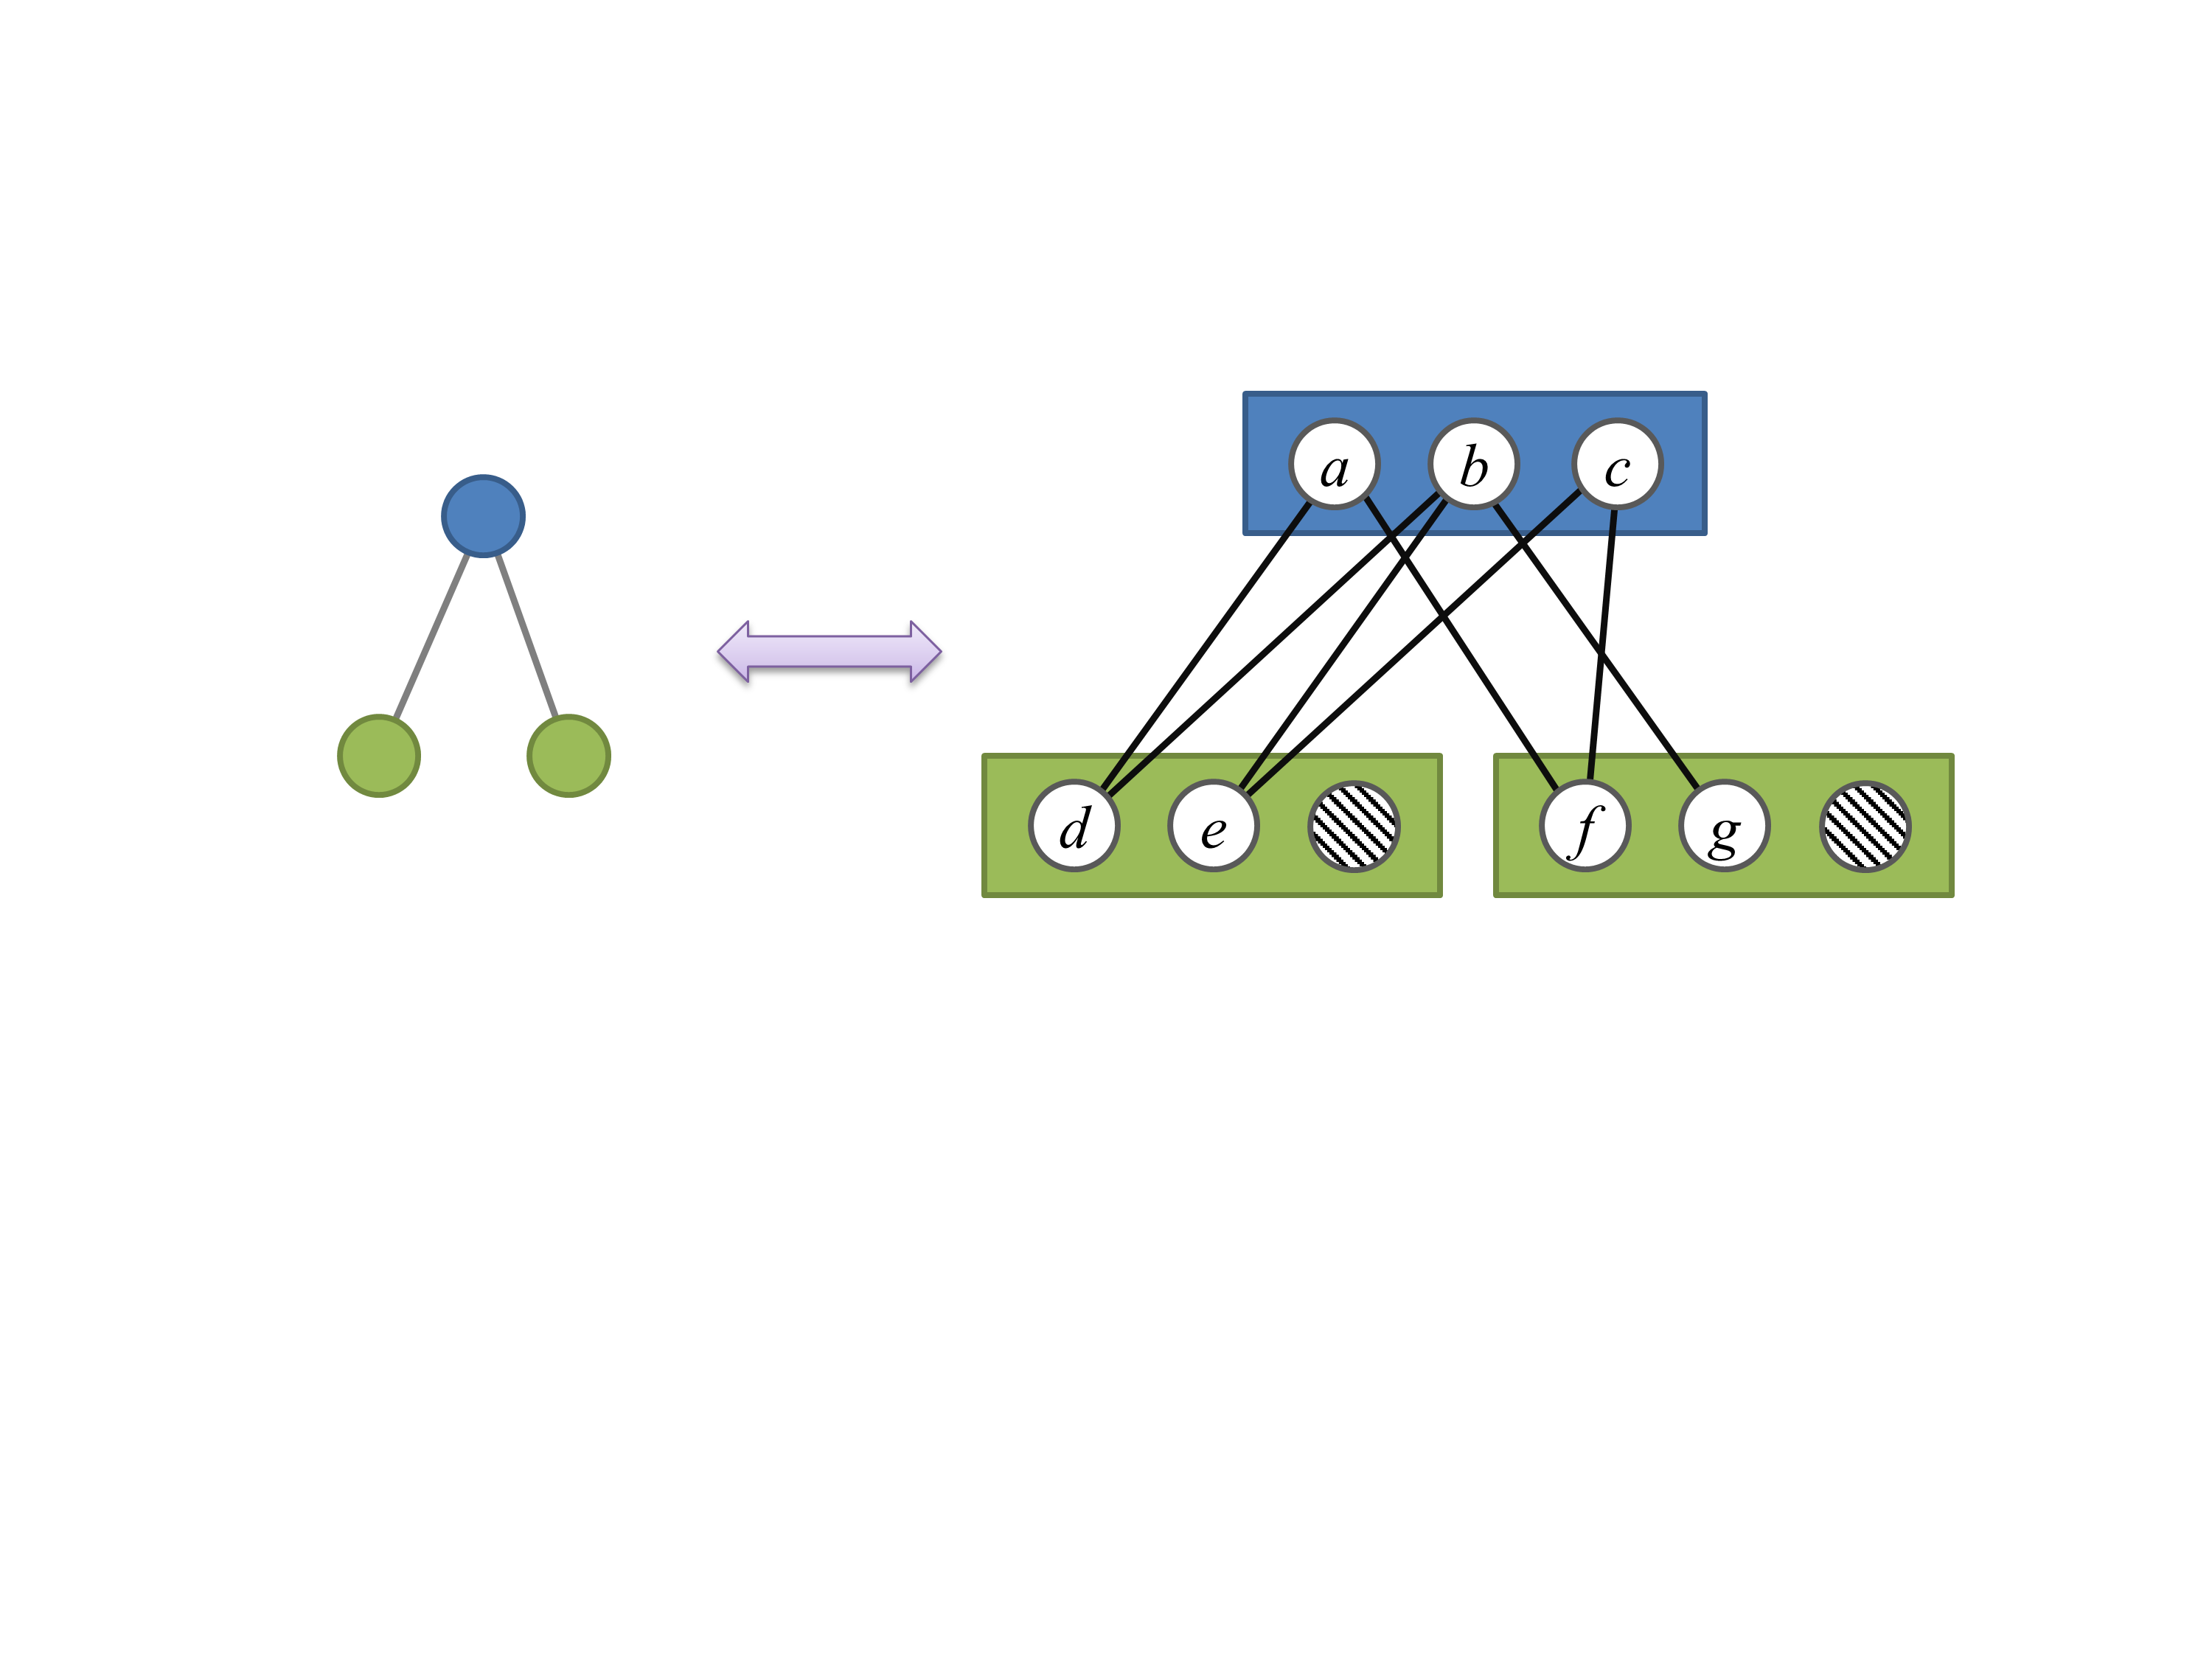
\includegraphics[trim={0 5cm 0 0}, clip, width=1.15\linewidth]{figure/Planar/Slide1.PNG}
   %\caption{{\sc Split}} \label{fig:split}
%\end{minipage}%
%\begin{minipage}{.5\textwidth}
  %\centering
   %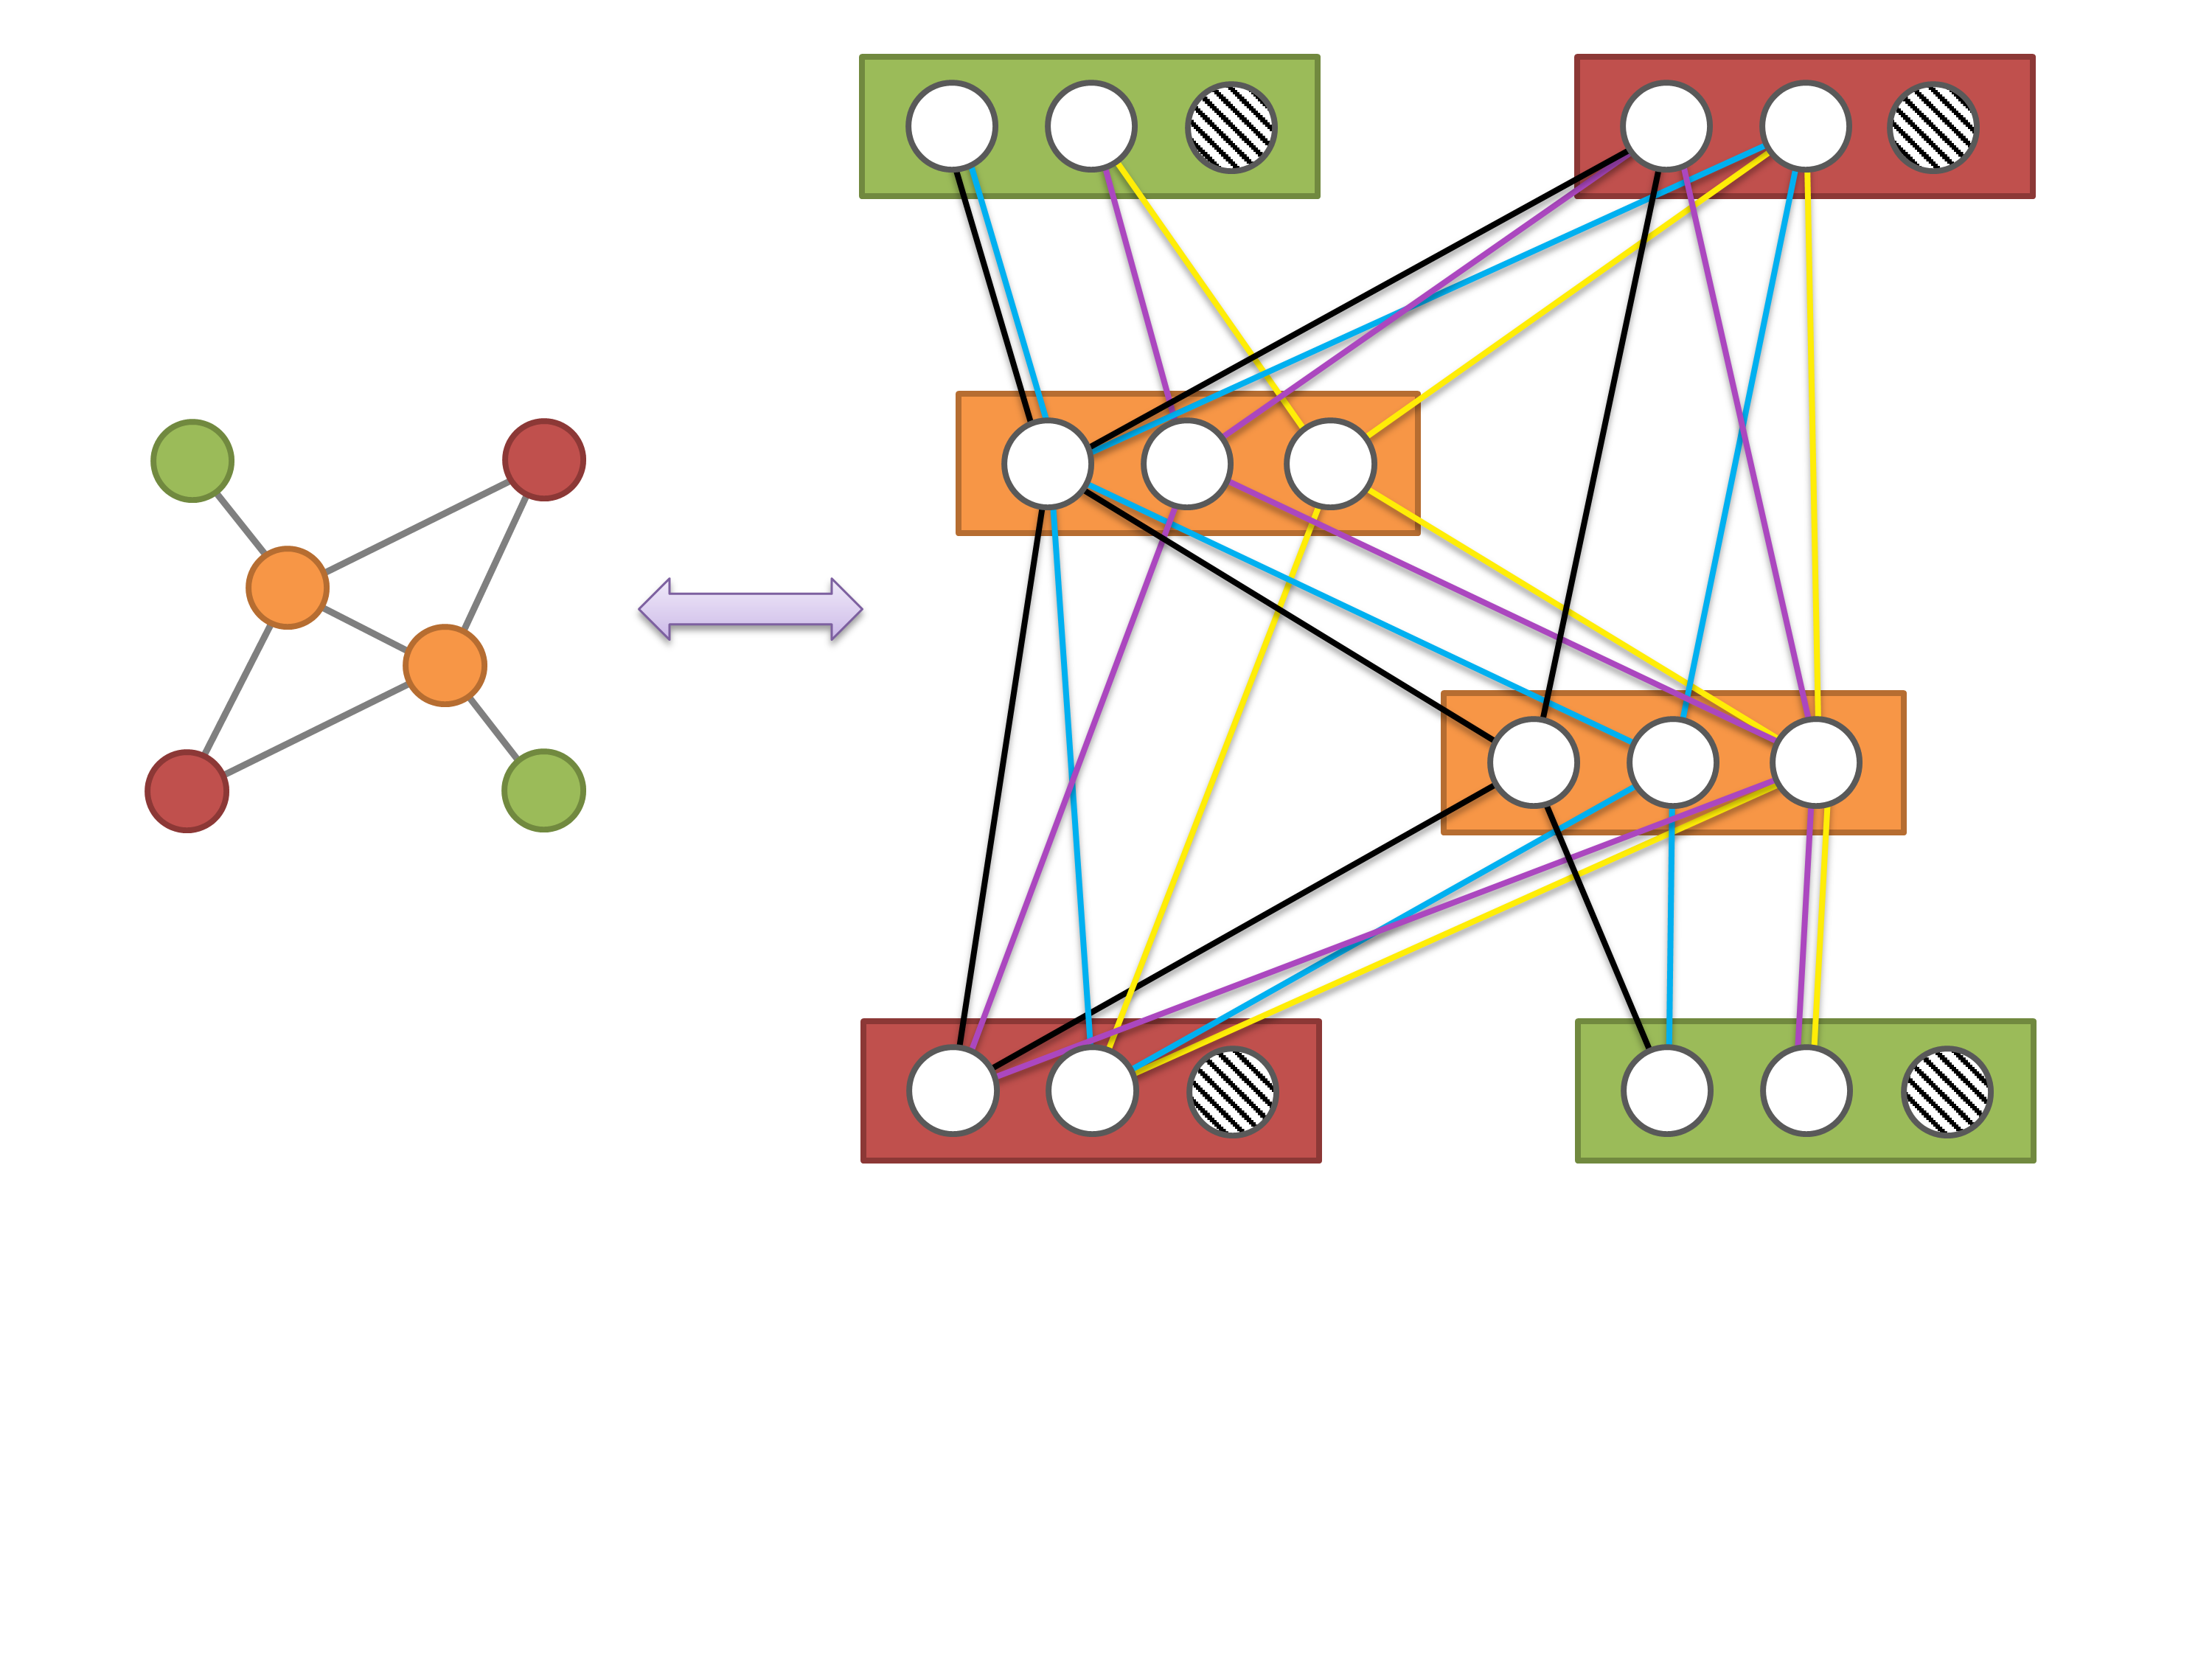
\includegraphics[trim={0 5cm 0 0}, clip, width=1.15\linewidth]{figure/Planar/Slide2.PNG}
   %\caption{{\sc UncrossCopy} } \label{fig:uncrosscopy}
%\end{minipage}
%\end{figure}

% 
The two gadgets used in our reduction are illustrated in Figure~\ref{fig:split}. A 3-label node can be encoded as a collection of 3 indicator variables with a one-hot constraint. In the figure, a solid colored circle denotes a 3-label node, and a solid colored rectangle denotes the equivalent node expressed with indicator variables (white circles).  For example, in Figure~\ref{fig:split}, $a=1$ corresponds to the blue node taking the first label value. The pairwise potentials (edges on the left part of the figures) can be viewed as edge costs between the indicator variables (black lines on the right), \eg, $f_{uv}(3, 2)$ is placed onto the edge between indicator $c$ and $e$ and is counted into the overall measure if and only if $c = e = 1$. In our gadgets, drawn edges represent zero cost while omitted edges represent positive infinity\footnote{A very large number will also serve the same purpose, \eg, take the sum of the absolute value of all energy terms and add 1. Therefore, we are not expanding the set of allowed energy terms to include $\infty$.}.  While the set of feasible solutions remains the same, the gadget encourages certain labeling relationships, which, if not satisfied, cause the overall measure to be infinity. Therefore, the encouraged relationships must be satisfied by any optimal solution. The two gadgets serves different purposes:

\textsc{Split} A 3-label node (blue) is split into two 2-label nodes (green). The shaded circle represents a label with a positive infinite unary cost and thus creates a simulated 2-label node. The encouraged relationships are
\begin{itemize}
    \item $a = 1 \leftrightarrow d = 1 \text{ and } f = 1$.
    \item $b = 1 \leftrightarrow g = 1$.
    \item $c = 1 \leftrightarrow e = 1 \text{ and } f = 1$.
\end{itemize}
Thus $(d,f)$ encodes $a$, $(d,g)$ and $(e,g)$ both encode $b$ and $(e,f)$ encodes $c$.

\textsc{UncrossCopy} The values of two 2-label nodes are encouraged to be the same as their diagonal counterparts respectively (red to red, green to green) without crossing with each other. The orange nodes are intermediate nodes that pass on the values. All types of lines represent the same edge cost, which is 0. The color differences visualize the verification for each of the 4 possible states of two 2-label nodes.  For example, the cyan lines verify the case where the top-left (green) node takes the values (1, 0) and the top-right (red) node takes the value (0, 1).  It is clear that the encouraged solution is for the bottom-left (red) node to take the value (0, 1), and the bottom-right (green) node to take the value (1, 0).

\begin{figure}[t]
\centering
\begin{tabular}{cc}
\begin{tabular}{c}%
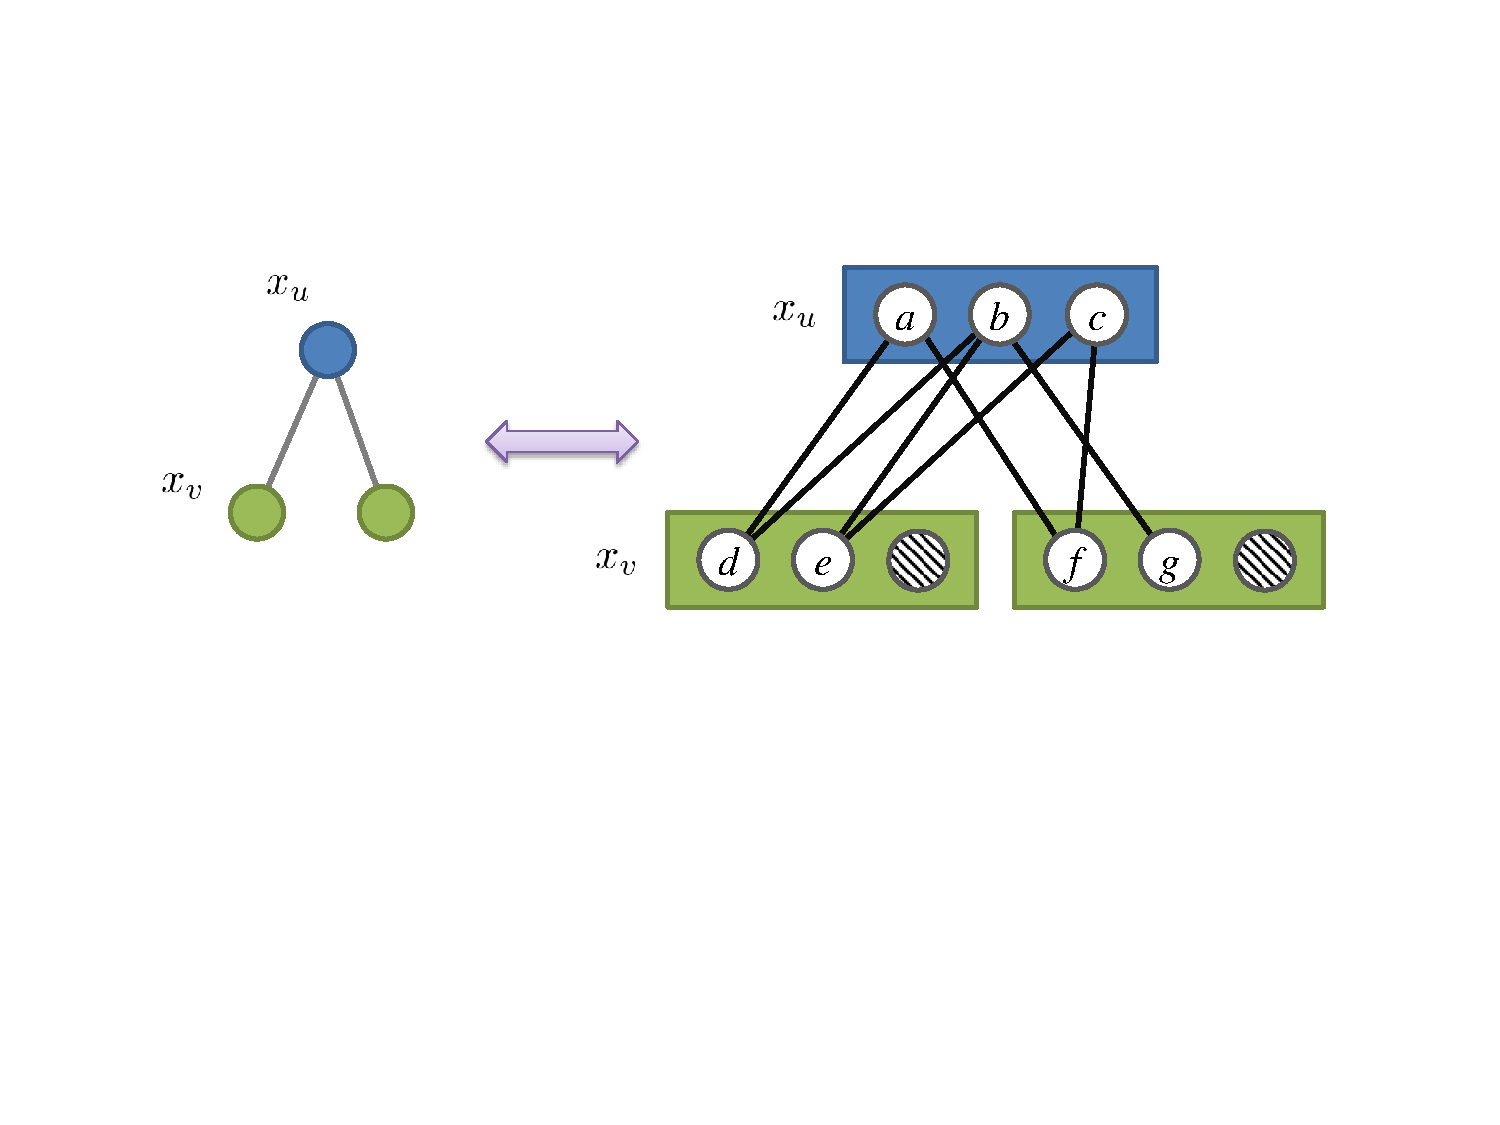
\includegraphics[width=0.39\linewidth]{figure/Planar/Planar-1-crop.pdf}
\end{tabular}&\ \ \ \ \ \ 
\begin{tabular}{c}%
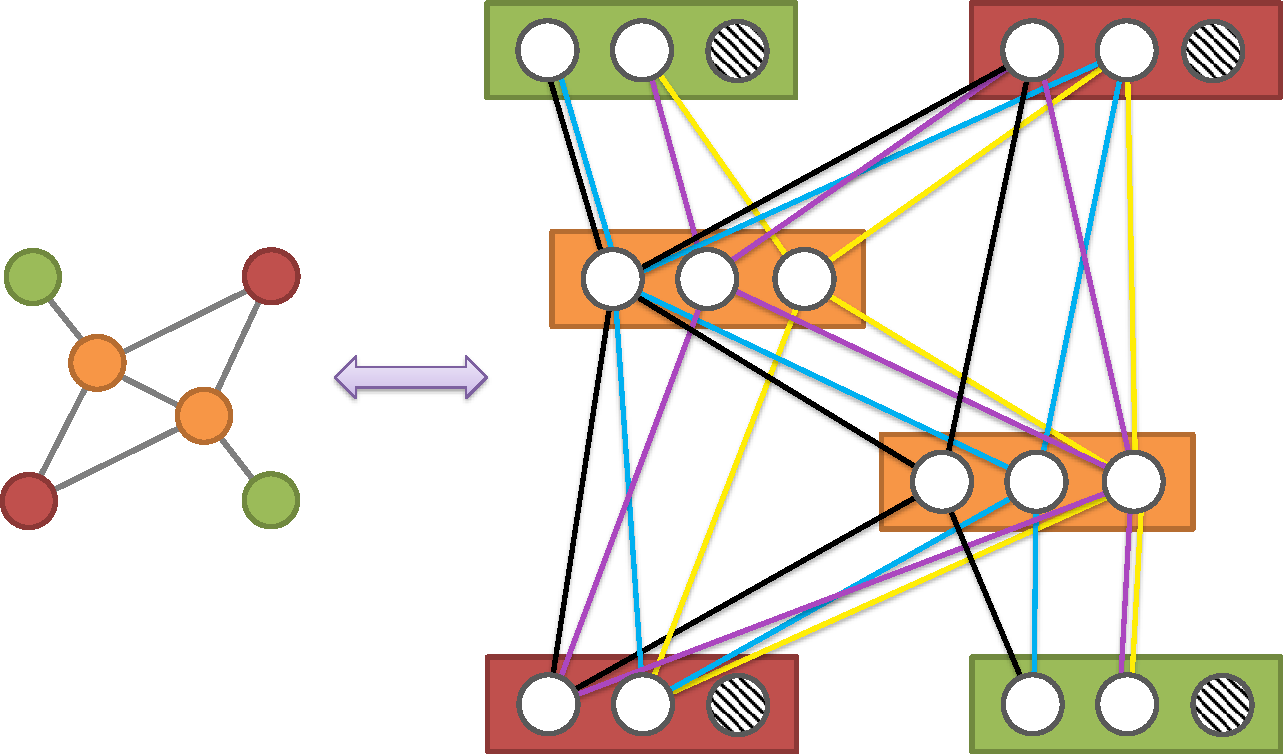
\includegraphics[width=0.39\linewidth]{figure/Planar/Planar-2-crop.pdf}
\end{tabular}\\
{\sc Split} & {\sc UncrossCopy}
\end{tabular}
\caption{Gadgets to represent a 3-label variable as two 2-label variables ({\sc Split}) and to copy the values of two diagonal pairs of 2-label variables without edge crossing ({\sc UncrossCopy}).\label{fig:split}}
\end{figure}

\begin{figure}[b]
\begin{center}
   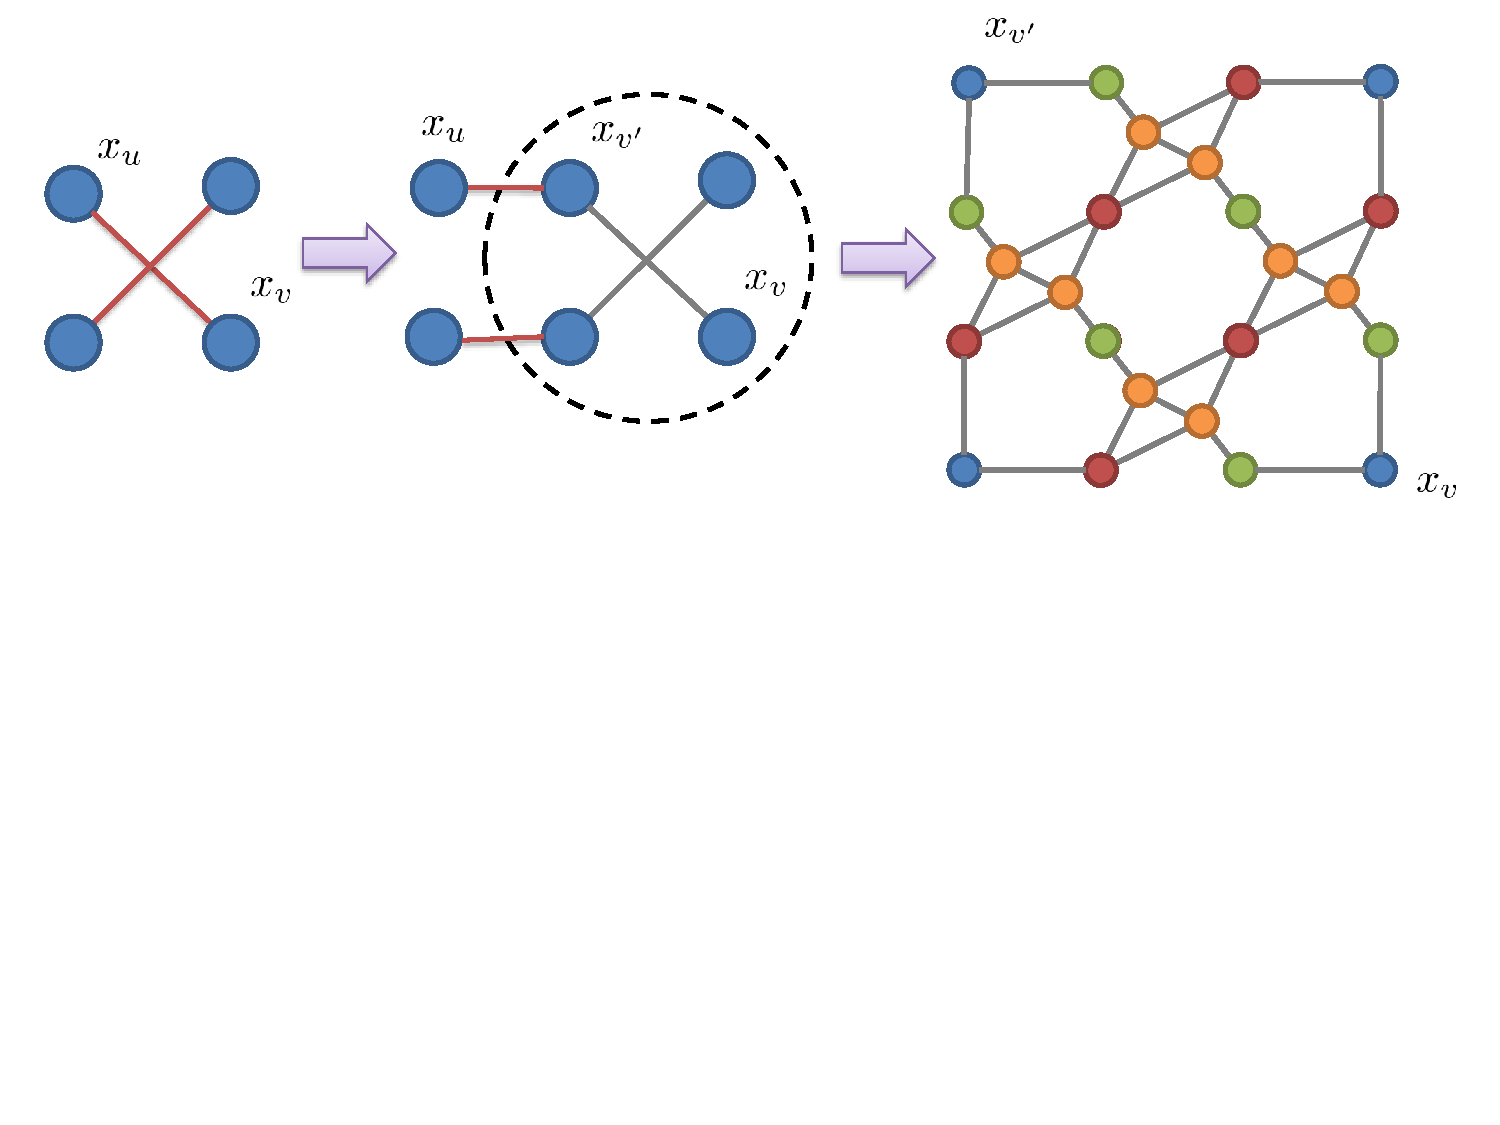
\includegraphics[trim={0 10.5cm 0 0}, clip, width=0.7\linewidth]{figure/Planar/Planar-3.pdf}
\end{center}
\caption{Planar reduction for 3-label problems} \label{fig:planarreduct}
\end{figure}

These two gadgets can be used to uncross the intersecting edges of two pairs of 3-label nodes (Figure~\ref{fig:planarreduct}, left).  For a crossing edge ($x_u$, $x_v$), first a new 3-label node $x_v'$ is introduced preserving the same arbitrary interaction (red line) as before (Figure~\ref{fig:planarreduct}, middle). Then, the crossing nodes (shown within the dotted circle) are uncrossed by applying {\sc Split} and {\sc UncrossCopy} four times (Figure~\ref{fig:planarreduct}, right).
Without loss of generality, we can assume that no more than two edges intersect at a common point except at their endpoints.  This process can be applied repeatedly at each edge crossing until there are no edge crossings left in the graph~\cite{prusa2015universality}.
